\begin{center}
\Huge
Modeller
\end{center}
\section*{Modeller}
\stepcounter{section}

Vi skal arbejde med modeller, og I har selv læst og skrevet lidt om, hvad modeller er i matematik. Generelt forestiller vi os, at vi har en virkelig problemstilling, som vi godt vil bruge matematik til at løse. Vi opsamler så data eller overvejer, hvordan vi tror, at virkeligheden hænger sammen og prøver så at beskrive det som en matematisk problemstilling. Denne matematiske problemstilling kan vi forhåbentlig løse med nogle af de værktøjer, vi har i matematik. Denne løsning oversættes så tilbage til den virkelige problemstilling, vi så forhåbentlig kan løse ved hjælp af matematik. 


\begin{exa}
En virkelig problemstilling kan være at bestemme, om en mønt har lige stor sandsynlighed for at slå plat som krone. Vi antager derfor, at dette er tilfældet for vores mønt. Derfor vil et møntslag kunne beskrives med en Bernoulli-fordelt stokastisk variabel med sandsynlighedsparamer $p = 0,5$. Vi slår nu med mønten 100 gange og får plat 35 gange. Antallet af successer i disse 100 forsøg kan beskrives ved hjælp af en binomialfordelt stokastisk variabel med sandsynlighedsparameter $p = 0,5$ og antalsparameter $n = 100$. Vi laver så en tosidet binomialtest for at se, hvad sandsynligheden for at få et lige så eller mere ekstremt udfald end $k = 35$. Signifikansniveauet sættes til $0.05$. Dette gøres i Maple, og resultatet kan ses af Fig \ref{fig:bintest}
\begin{figure}[H]
\centering
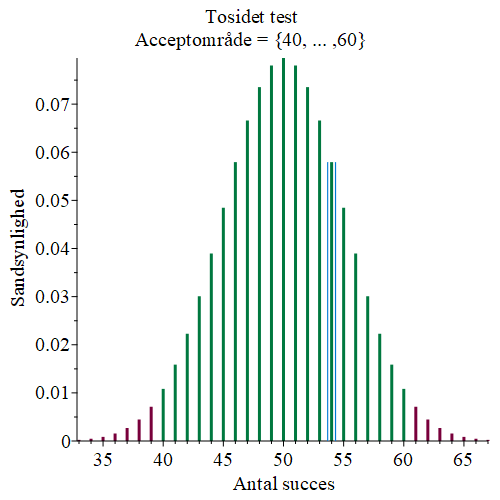
\includegraphics[width=\textwidth*3/4]{Billeder/Bintest.png}
\caption{Binomialtest med $n=100$, $p = 0.5$ og signifikansniveau $0.05$.}
\label{fig:bintest}
\end{figure}
Vi kan se, at acceptområdet er $\{ 40,...,60\}$, hvilket $35$ ikke ligger i. Derfor forkaster vi vores tro på, at mønten er fair. 

Med modellen kan vi regne på, hvorvidt vi vil tro på et givet udfald uden blot at skulle gisne. 
\end{exa}

\begin{exa}
Vi betragter bakterievækst i en opløsning. Vi måler følgende sammenhæng mellem tid og antal bakterier
\begin{center}
\begin{tabular}{c|c|c|c|c|c|c}
Tid (timer) & 1 & 2 & 3 & 4 & 5 & 6 \\ \hline 
Bakterier (mio) & 10.2 & 11.0 & 12.1 & 13.5 & 15.1 & 17.9
\end{tabular}
\end{center}
Vi vil forvente, at bakterievæksten i en begrænset periode kan beskrives ved eksponentiel vækst. Vi kan derfor lave eksponentiel regression på datasættet. Dette kan ses af Fig. \ref{fig:expreg}.
\begin{figure}[H]
\centering
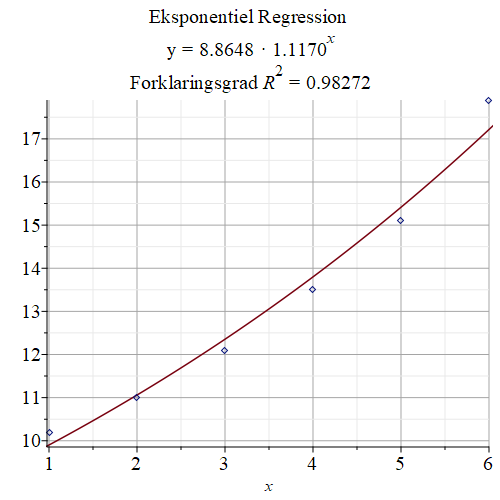
\includegraphics[width=\textwidth*3/4]{Billeder/expreg2.png}
\caption{Eksponentiel regression på bakteriedata}
\label{fig:expreg}
\end{figure}
Vi skal nu overveje, om denne model af væksten kan bruges til at beskrive væksten for evigt. Svaret er selvfølgelig nej, da pladsmangel, mangel på mad, ophobning af giftstoffer osv vil begrænse væksten og til sidst slå bakteriekolonien ihjel. En mere repræsentativ model for bakterievækst er den logistiske vækst. 
\end{exa}

\section*{Opgave 1}
Lad $M(x)$ beskrive vægten af et kvadratisk stykke papir med bredde $x$. Så er vægten givet ved
\begin{align*}
M(x) = k\cdot x^2
\end{align*}
for en given konstant $k$.
\begin{enumerate}[label=\roman*)]
\item Forklar, hvorfor vægten vokser kvadratisk som funktion af bredden.
\item Diskutér hvilke parametre $k$ bestemmes ad. 
\item En bestemt type papir vejer 100g per kvadratmeter. Sæt enheder på $x$ og $M(x)$ og bestem så $k$ for denne type papir.
\item Bestem vægten af et stykke papir med bredde $10cm$
\item Hvad er bredden af et papirkvadrat på $10kg$?
\end{enumerate}
\section*{Opgave 2}
Et supermarked har mistanke om, at lidt for mange af de æg, de modtager er knuste ved modtagelsen. Producenten lover, at $99\%$ af æggene er hele, når de når frem. Hvad skal butikken gøre for at afgøre deres mistanke? Blandt en stikprøve på 10.000 æg har de fundet 160 knuste æg. Undersøg, om butikken har grund til mistanke.

\section*{Opgave 3}
Ud fra tidligere erfaringer antager vi, at sammenhængen mellem antallet af solgte bøger og prisen på en bog er givet ved $(1200-x)$, hvor $x$ er prisen på bogen. Er bogen gratis, sælger vi $1200$, og koster den $1199$, så sælger vi én. Desuden koster det $200$kr at producere en bog, altså er fortjenesten per bog $x-200$. Derfor må omsætningen af bogen kunne beskrives ved
\begin{align*}
O(x) = (1200-x)(x-200) = -x^2+1400x-240000.
\end{align*}
\begin{enumerate}[label=\roman*)]
\item Bestem en graf for omsætningen $O(x)$. 
\item Optimér omsætningen ved brug af differentialregning. 
\end{enumerate}